\usetikzlibrary{patterns}


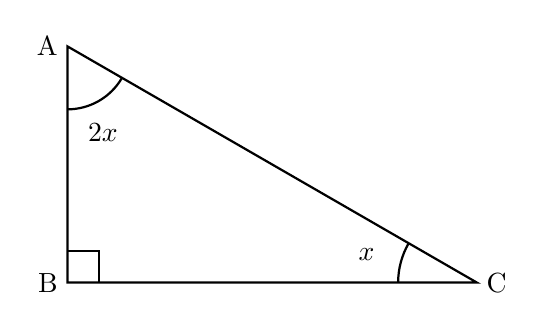
\begin{tikzpicture}[scale=1]

    % Define the coordinates for the vertices of the right-angled triangle
    % Using proportions of a 30-60-90 triangle (base = height * sqrt(3))
    \coordinate (A) at (0, 3);
    \coordinate (B) at (0, 0);
    \coordinate (C) at (5.2, 0); 

    % Draw the main triangle lines (AB, BC, CA)
    \draw[thick] (A) -- (B) -- (C) -- cycle;

    % Draw the right-angle square symbol at vertex B
    \draw[thick] (0.4, 0) -- (0.4, 0.4) -- (0, 0.4);

    % Draw the arc for angle 2x at vertex A
    % The arc starts from the vertical line AB (-90 degrees) to the hypotenuse AC (-30 degrees)
    \draw[thick] (0, 2.2) arc (-90:-30:0.8);

    % Draw the arc for angle x at vertex C
    % The arc starts from the horizontal line BC (180 degrees) to the hypotenuse AC (150 degrees)
    \draw[thick] (4.2, 0) arc (180:150:1.0);

    % Label the vertices exactly as shown in the image
    \node[left] at (A) {A};
    \node[left] at (B) {B};
    \node[right] at (C) {C};

    % Place the angle measurements (2x and x)
    \node at (0.45, 1.9) {$2x$};
    \node at (3.8, 0.35) {$x$};

\end{tikzpicture}